% 图 6.30 封闭畴示意：四条主畴 + 顶底三角封闭畴，标 D 与 L
\documentclass[tikz,border=5pt]{standalone}
\usetikzlibrary{arrows.meta}
\usepackage{amsmath}
\usepackage{bm}
\usepackage{fontspec}
\setmainfont{Times New Roman}
\begin{document}
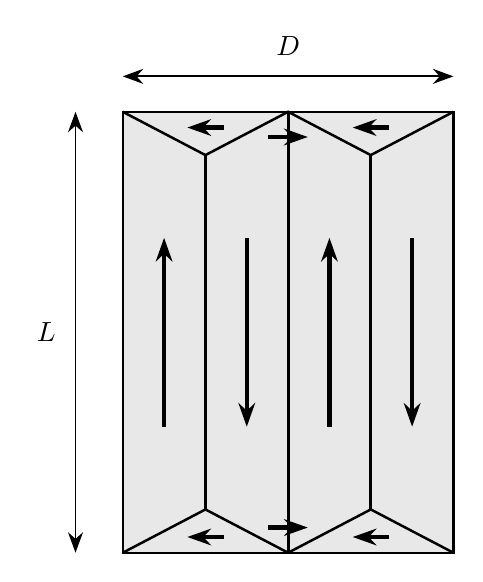
\begin{tikzpicture}[line width=0.8pt,>=Stealth,
  mag/.style={->,line width=1.5pt,>={Stealth[length=3mm,width=2.1mm]}},
  dim/.style={<->,line width=0.7pt,>={Stealth[length=2.6mm,width=1.9mm]}}]
% sample rectangle
\fill[gray!18] (0,0) rectangle (4.2,5.6);
\draw[line width=0.9pt] (0,0) rectangle (4.2,5.6);
% main domain walls
\draw[line width=1.1pt] (1.05,0.55) -- (1.05,5.05);
\draw[line width=1.1pt] (2.1,0) -- (2.1,5.6);
\draw[line width=1.1pt] (3.15,0.55) -- (3.15,5.05);
% closure slant walls (top)
\draw[line width=0.9pt] (0,5.6) -- (1.05,5.05) -- (2.1,5.6) -- (3.15,5.05) -- (4.2,5.6);
% closure slant walls (bottom)
\draw[line width=0.9pt] (0,0) -- (1.05,0.55) -- (2.1,0) -- (3.15,0.55) -- (4.2,0);
% main domain arrows: up down up down
\draw[mag] (0.525,1.6) -- (0.525,4.0);
\draw[mag] (1.575,4.0) -- (1.575,1.6);
\draw[mag] (2.625,1.6) -- (2.625,4.0);
\draw[mag] (3.675,4.0) -- (3.675,1.6);
% closure arrows top: left right left
\draw[mag] (1.28,5.4)  -- (0.82,5.4);
\draw[mag] (1.85,5.28) -- (2.35,5.28);
\draw[mag] (3.38,5.4)  -- (2.92,5.4);
% closure arrows bottom: left right left
\draw[mag] (1.28,0.2)  -- (0.82,0.2);
\draw[mag] (1.85,0.32) -- (2.35,0.32);
\draw[mag] (3.38,0.2)  -- (2.92,0.2);
% D (width) and L (height) annotations
\draw[dim] (0,6.05) -- (4.2,6.05);
\node[anchor=south] at (2.1,6.18) {$D$};
\draw[dim] (-0.6,0) -- (-0.6,5.6);
\node[anchor=east] at (-0.72,2.8) {$L$};
\end{tikzpicture}
\end{document}
